\documentclass{article}

\usepackage[left=2cm,right=2cm,top=2cm,bottom=2cm]{geometry}
\usepackage{graphicx}
\usepackage{xspace}

\newcommand{\hangout}{\textsc{Google Hangout}\xspace}
\newcommand{\host}{\textsc{PuzzleHost}\xspace}
\newcommand{\speaker}{\textsc{PuzzleSpeaker}\xspace}

\title{\textbf{Standard Operating Procedure for Conducting Successful} \textsc{Google Hangout}}
\author{Puzzles}

\date{Last update: \today}

\begin{document}

\maketitle

\begin{abstract}
Currently, all communication and training sessions in Puzzles are carried out through \hangout. This article presents a Standard Operating Procedure (SOP) for conducting a successful \hangout session. All procedures have to be followed by host of \hangout session. This documentation is not to explain recording plans.
\end{abstract}

\tableofcontents

\clearpage
\section{Host}

\paragraph{1.1} All public \hangout sessions are hosted on the behalf of Amy Theia Knuth (referred as Amy here and after).

\paragraph{1.2} Amy is accessible through:
\begin{verbatim}
http://google.com/+AmyKnuthTheia/
\end{verbatim}

\paragraph{1.3} Amy is reachable through:
\begin{verbatim}
amy.theia.knuth@gmail.com
\end{verbatim}

\paragraph{1.4} Only limited number of Puzzlers have access to Amy's account. They are referred as \host here and after. The list is maintained by Amy.

\paragraph{1.5} Password of Amy's account can not be changed.

\paragraph{1.6} \host can gain access to Amy's account by emailing to Amy.

\paragraph{1.7} \host is not allowed to distribute Amy's password publicly.

\paragraph{1.8} If the \host can not perform the duty of hosting a \hangout session, the \host shall find another \host to perform the duty or call off the \hangout session.

\paragraph{1.9} \host schedules, organizes and conducts \hangout.

\paragraph{1.10} \host is advised that he/she shall not expect profit of any forms from the \hangout.

\clearpage
\section{Speaker}

\paragraph{2.1} Speaker is the person who presents materials of a \hangout. They are referred as \speaker here an after.

\paragraph{2.2} \speaker is appointed by \host of the \hangout. \speaker does not have to be a member of Puzzles.

\paragraph{2.3} If the \speaker can not perform the duty of presenting, the \host is allowed to make the decision whether changing the speaker or reschedule the \hangout.

\paragraph{2.4} \speaker is solely responsible for his/her own presentation and manner of speaking.

\paragraph{2.5} \speaker is advised that he/she shall not expect profit of any forms from the \hangout.

\clearpage
\section{Preparation} \label{sec:prepare}

\paragraph{\ref{sec:prepare}.1} If \host does not have password to Amy's account, he/she shall email to Amy for requesting the password.

\paragraph{\ref{sec:prepare}.2} \host logs in Amy's \texttt{Google+} profile.

\paragraph{\ref{sec:prepare}.3} \host starts to schedule an \hangout by clicking ``Start a Hangout On Air''.

\begin{figure}[!htm]
\centering
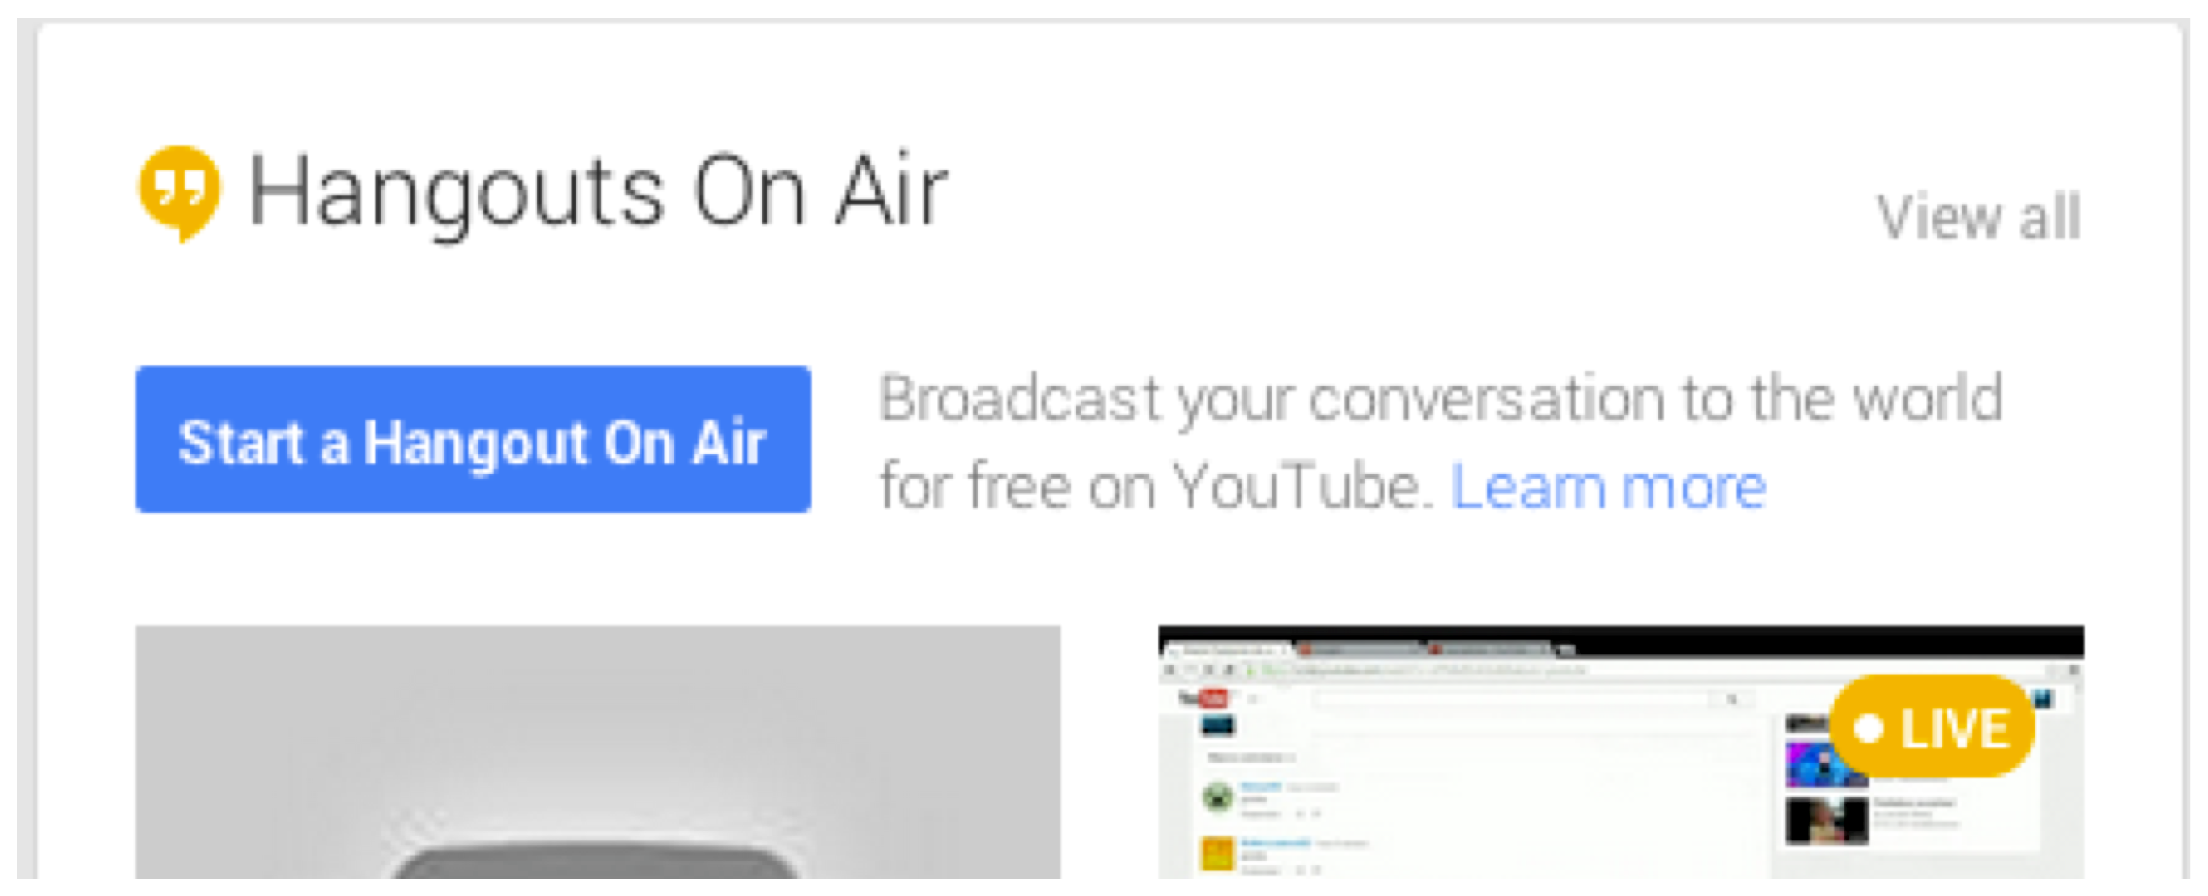
\includegraphics[width=0.35\textwidth]{images/sop_start_hangout.eps}
\end{figure}

\paragraph{\ref{sec:prepare}.4} \host fills up \hangout name, description, time. \host invites \speaker, public and certain Puzzles circle as audience. \hangout name is determined by Puzzles running series. The description has to include following line.

\emph{If you have any question, please send email to Amy Theia Knuth (\texttt{amy.theia.knuth@gmail.com})}

\paragraph{\ref{sec:prepare}.5} The \hangout has to be scheduled at least \textbf{3} days before the \hangout.

\clearpage
\section{Conduct \hangout} \label{sec:conduct}

\paragraph{\ref{sec:conduct}.1} \host is assumed that he/she has logged in Amy's \texttt{Google+} account and opened the scheduled \hangout event page.

\paragraph{\ref{sec:conduct}.2} \host clicks ``Start'' to start the hangout session.

\begin{figure}[!htm]
\centering
\includegraphics[width=0.35\textwidth]{images/sop_start_button.eps}
\end{figure}

\paragraph{\ref{sec:conduct}.3} \host invites \speaker and audiences before entering \hangout room.

\begin{figure}[!htm]
\centering
\includegraphics[width=0.6\textwidth]{images/sop_invite.eps}
\end{figure}

\paragraph{\ref{sec:conduct}.4} \host cuts off his/her camera and microphone once he/she enters \hangout room.

\paragraph{\ref{sec:conduct}.5} \host cuts off all audiences camera and microphone. This condition is kept till the broadcast is stopped.

\paragraph{\ref{sec:conduct}.6} \speaker's camera and microphone has to be on through entire \hangout.

\paragraph{\ref{sec:conduct}.7} \host confirms audio and video quality with \speaker and audiences.

\paragraph{\ref{sec:conduct}.8} \host clicks ``Start broadcast'' when \speaker is ready. Starting broadcast needs several seconds.

\begin{figure}[!htm]
\centering

\includegraphics[width=0.35\textwidth]{images/sop_start_broadcast.eps}
\end{figure}

\paragraph{\ref{sec:conduct}.9} \speaker starts to present once ``OFF AIR'' sign on the top right corner turns to ``LIVE''.

\begin{figure}[!htm]
\centering
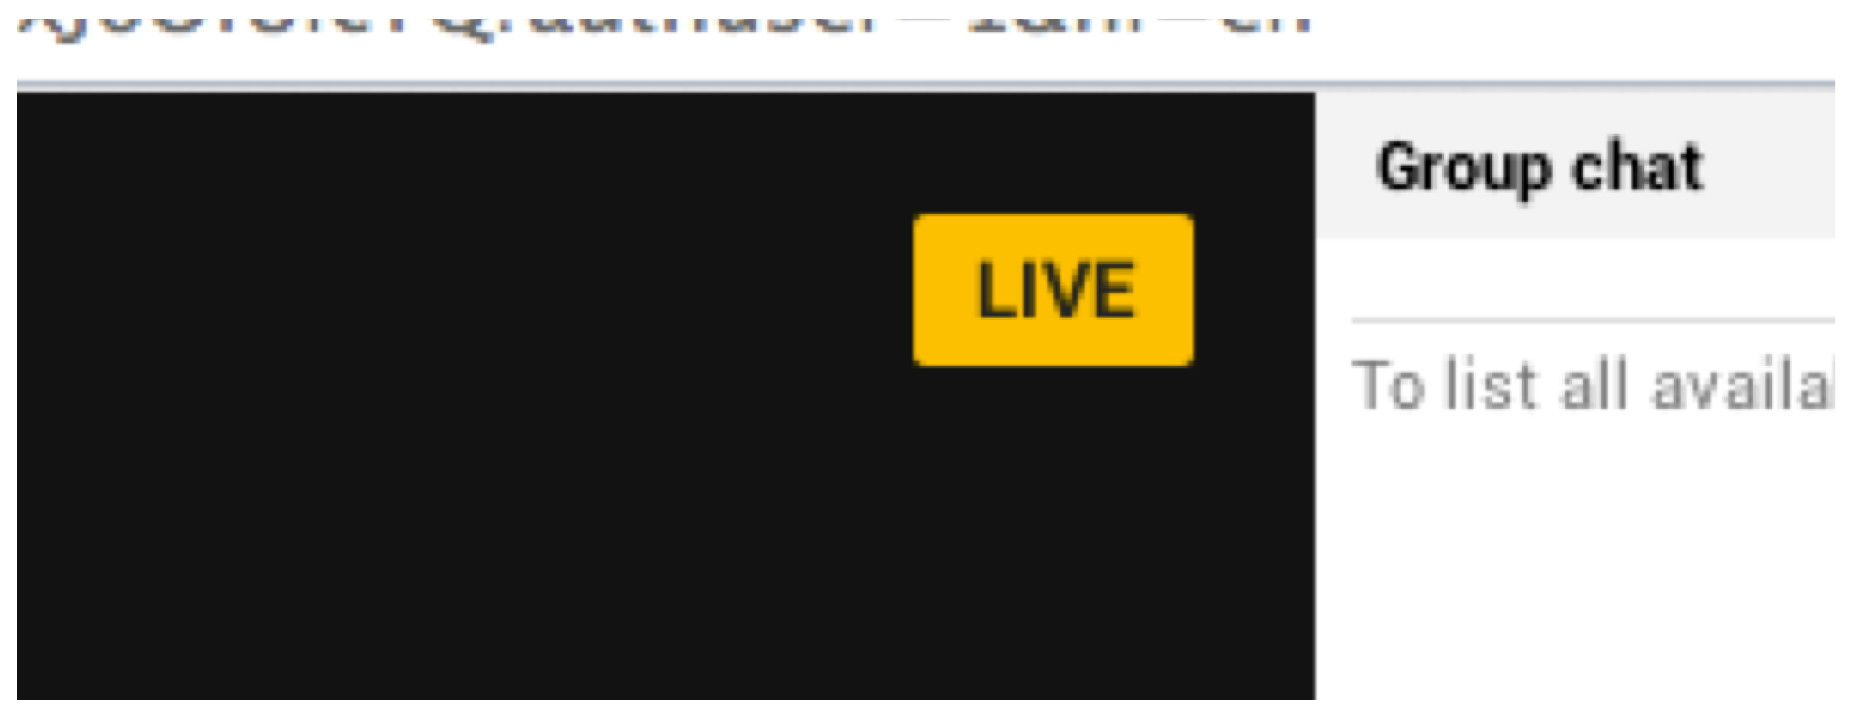
\includegraphics[width=0.35\textwidth]{images/sop_live.eps}
\end{figure}

\paragraph{\ref{sec:conduct}.10} \host clicks ``Stop broadcast'' when \speaker indicates the end of presentation.

\begin{figure}[!htm]
\centering

\includegraphics[width=0.35\textwidth]{images/sop_stop_broadcast.eps}
\end{figure}

\paragraph{\ref{sec:conduct}.11} \speaker stops talking when \hangout is off air.

\paragraph{\ref{sec:conduct}.12} \host is allowed to un-mute audience when broadcast is stopped.

\paragraph{\ref{sec:conduct}.13} \host is allowed to leave the \hangout when broadcast is stopped.

\paragraph{\ref{sec:conduct}.14} \host is allowed to make decision when the \hangout meets technical problems in any forms.

\clearpage
\section{After \hangout} \label{sec:end}

\paragraph{\ref{sec:end}.1} The hangout record is available at \texttt{YouTube} as soon as \host leaves the \hangout. (Due to delay of \texttt{YouTube}, \host checks the record on \texttt{YouTube} in every 20 minutes for ensuring that video record is saved to Amy's \texttt{YouTube} channel.)

\paragraph{\ref{sec:end}.2} All \hangout records are saved and managed in Amy's \texttt{YouTube} channel:
\begin{verbatim}
http://www.youtube.com/channel/UCLApsra6s1A7IrDefL472-g
\end{verbatim}

\paragraph{\ref{sec:end}.3} \host added the \hangout record to the corresponding play list.

\paragraph{\ref{sec:end}.4} \host will be notified if there is any changes on the \hangout record.

\paragraph{\ref{sec:end}.5} A \hangout record will be replaced under following two circumstances:
\begin{itemize}
	\item An updated version is approved by Amy.
	\item The record is not usable under technical errors.
\end{itemize}

\end{document}